\documentclass[5p]{elsarticle}
\usepackage{subfig}
\usepackage{lineno,hyperref}
\usepackage{amsmath}
\usepackage{algorithm}
\usepackage{lipsum}
\usepackage{multirow}
\usepackage[noend]{algpseudocode}
\usepackage{graphicx}
\renewcommand{\algorithmicrequire}{\textbf{Input:}}
\renewcommand{\algorithmicensure}{\textbf{Output:}}
\modulolinenumbers[5]
\newdefinition{definition}{Definition}

\journal{Journal of \LaTeX\ Templates}

%%%%%%%%%%%%%%%%%%%%%%%
%% Elsevier bibliography styles
%%%%%%%%%%%%%%%%%%%%%%%
%% To change the style, put a % in front of the second line of the current style and
%% remove the % from the second line of the style you would like to use.
%%%%%%%%%%%%%%%%%%%%%%%

%% Numbered
%\bibliographystyle{model1-num-names}

%% Numbered without titles
%\bibliographystyle{model1a-num-names}

%% Harvard
%\bibliographystyle{model2-names.bst}\biboptions{authoryear}

%% Vancouver numbered
%\usepackage{numcompress}\bibliographystyle{model3-num-names}

%% Vancouver name/year
%\usepackage{numcompress}\bibliographystyle{model4-names}\biboptions{authoryear}

%% APA style
%\bibliographystyle{model5-names}\biboptions{authoryear}

%% AMA style
%\usepackage{numcompress}\bibliographystyle{model6-num-names}

%% `Elsevier LaTeX' style
\bibliographystyle{elsarticle-num}
%%%%%%%%%%%%%%%%%%%%%%%

\begin{document}

	\begin{frontmatter}

		\title{RejectMIDAS: Microcluster-Based Detector of Anomalies with Rejection\tnoteref{t1}}
		\tnotetext[t1]{Code, datasets and experiment results are published at \href{https://github.com/liurui39660/RejectMIDAS}{https://github.com/liurui39660/RejectMIDAS}.}

%% Group authors per affiliation:
%		\author{Elsevier\fnref{myfootnote}}
%		\address{Radarweg 29, Amsterdam}
%		\fntext[myfootnote]{Since 1880.}

%% or include affiliations in footnotes:
%		\author[mymainaddress,mysecondaryaddress]{Elsevier Inc}
%		\ead[url]{www.elsevier.com}

%		\author[mysecondaryaddress]{Global Customer Service\corref{mycorrespondingauthor}}
%		\cortext[mycorrespondingauthor]{Corresponding author}
%		\ead{support@elsevier.com}

%		\address[mymainaddress]{1600 John F Kennedy Boulevard, Philadelphia}
%		\address[mysecondaryaddress]{360 Park Avenue South, New York}

		\author[1]{Rui Liu}
		\ead{liurui@comp.nus.edu.sg}

		\author[1]{Bryan Hooi\corref{CA}}
		\ead{dcsbhk@nus.edu.sg}

		\cortext[CA]{Corresponding author.}

		\address[1]{School of Computing, National University of Singapore, Singapore}

		\begin{abstract}
			In 2020, Bhatia et al. proposed the MIDAS algorithm. Their algorithm processes edge streams and produces an anomaly score for each edge. It is simple but fast and accurate. However, there is a loophole in this algorithm that if the anomalous situation persists, e.g., a denial of service attack lasts for a day, the algorithm will gradually get accustomed to this situation, and produces underestimated scores for future anomalous edges.

			In this work, we propose our RejectMIDAS algorithm, which uses a threshold to prevent obviously anomalous edges from being merged into the internal states and affecting the resulting score. We simplified the anomaly score, and also introduce extra steps to reject the negative effects of anomalous edges. Though additional time complexity is introduced for clearing buffers, experiments show that if properly configured, the algorithm can achieve a better result while still have comparable running speed with the original version.

		\end{abstract}

%		\begin{keyword}
%			\texttt{elsarticle.cls}\sep \LaTeX\sep Elsevier \sep template
%			\MSC[2010] 00-01\sep  99-00
%		\end{keyword}

	\end{frontmatter}

	\linenumbers


	\section{Introduction}\label{sec:Introduction}

	Anomaly detection, also known as outlier detection, is a series of methods that detect data records whose attributes, distribution, or the number of occurrences are significantly different from the majority of data. Usually, these records correspond to varies kinds of malicious behaviors, such as scams, manipulations, or saturation attacks.

	Anomaly detection is a well-explored field where many established approaches can efficiently resolve the problem. However, some researches only focus on static graphs, which failed to capture the changes that happen in the real world. Therefore, these methods may miss the temporal relations and information of the existing data, and as a result, overlook the underlying perceptions and distributions.

	In 2020, Bhatia et al. proposed microcluster-based detector of anomalies in edge streams, a.k.a. MIDAS algorithm~\cite{bhatia2020midas}. Compared with other anomaly detection algorithms on graphs, their method has several advantages. Their algorithm utilizes two fixed-size count-min sketches (CMS)~\cite{cormode2005an} to maintain states within and across timestamps and has a constant time complexity for the processing of each incoming edge.

	However, from another side, there are still some problems in their algorithm, the most obvious one is that though the algorithm detects anomalies and gives a score to each edge, it keeps all the edges to the CMS without differentiating normal or anomalous ones. This behavior leads to a potential issue. Since one of the characteristics of anomalous edges is they usually approach the system in a burst, i.e., a large number of edges in a relatively short period, when the system is under attack, after giving a high anomaly score, the algorithm merges those edges into the internal states. Therefore, it is likely in the future, edges of the same type are regarded as normal. We will discuss this in detail in Sec.~\ref{sec:ProposedMethod}.


	\section{Related Works}\label{sec:RelatedWorks}

	In this section, we will briefly review the existing methods to detect anomalous data on static or dynamic graphs. See~\cite{akoglu2015graph} for a more comprehensive comparison and evaluation on graph-based anomaly detection algorithms.

	Anomaly detection in static graphs can be summarized into three categories: anomalous node detection, anomalous edge detection, and anomalous subgraph detection.

	Anomalous node detection: OddBall~\cite{akoglu2010oddball} is an anomaly detection algorithm on weighted graphs. It extracts four features, i.e., degree, number of edges, total weight, and principal eigenvalue, from graph nodes and group them into three pairs, then utilizing four empirical power laws to identify the irregular behavior of anomalous nodes. CatchSync~\cite{jiang2016catching} exploits two tell-tale signs, i.e., synchronized behavior and irregular connectivity, of the anomalous users. The authors then devise a new measure to qualify those concepts, and use the proposed algorithm to produce the synchronicity-normality plots to help highlight the anomalous nodes.

	Anomalous edge detection: AutoPart~\cite{chakrabarti2004autopart} is a parameter-free method that first groups nodes in the adjacency matrix into several clusters, encoding the graph base on the similar connectivity between nodes, then tries to find edges whose removal can significantly reduce the compression cost, so as to spot the anomalous edges. NrMF~\cite{tong2011non}, which stands for the non-negative residual matrix factorization framework, is a method that factorizes the adjacency matrix and then flags edges with high reconstruction error as outliers.

	Anomalous subgraph detection: FRAUDAR~\cite{hooi2017graph} is an algorithm that targets camouflaged fraudsters and hijacked accounts. It utilizes the priority tree to efficiently and repeatedly removes the least suspicious nodes, so as to identify the most anomalous subgraph. Shin et al.~\cite{shin2018patterns} explore three patterns: mirror pattern, core-triangle pattern, and structured core pattern. Based on the three patterns, they propose their algorithm to measures the deviation, then identifies the anomalous subgraph.

	Anomaly detection in dynamic graphs can also be divided into three types: for nodes, for edges, and for subgraphs.

	Anomalous node detection: DTA and STA~\cite{sun2006beyond} target high order data, like tensors; they approximate the adjacency matrix of the current snapshot based on incremental matrix factorization. Then, it spots nodes corresponding to rows with high reconstruction error. HotSpot~\cite{yu2013on} is a dynamic PCA-based method; it tracks the local correlation information, and detect nodes with sudden and significant changes.

	Anomalous edge detection: Ranshous et al.~\cite{ranshous2016a} propose three scores: sample score, preferential attachment score, and homophily score. Then uses the linear combination of them to spot anomalous edges in an edge stream. SedanSpot~\cite{eswaran2018sedanspot} is an algorithm that detects anomalies based on edge occurrence, preferential attachment and mutual neighbors. MIDAS~\cite{bhatia2020midas} uses count-min sketches (CMS) for counting the edge occurrence and a formula derived from $\chi^2$ goodness-of-fit as the anomaly score, to process an incoming edge stream and output a score for each edge.

	Anomalous subgraph detection: CopyCatch~\cite{beutel2013copycatch} uses clustering algorithm to spot anomalies on bipartite-like graphs, like the user-post graph. M-Zoom and M-Biz~\cite{shin2018fast} detect dense-subtensors with different density measures; they guarantee the density and the local optimality of the detected subtensors, respectively. DenseAlert~\cite{shin2017densealert} is an incremental algorithm that detects bursts of dense sub-tensors.


	\section{Preliminaries}

	\subsection{Notations}

	Table~\ref{tab:Notation} gives the list of symbols used in this paper.

	\begin{table}[h]
		\centering
		\caption{Notations}
		\label{tab:Notation}
		\begin{tabular}{cl}
			\hline
			Symbol & Definition \\
			\hline
			$a_{sub}$ & Count of edge/node $sub$ at current timestamp \\
			$b$ & Number of buckets (columns) in a CMS row \\
			$c_{sub}$ & Anomaly score for edge/node $sub$ \\
			$h$ & Number of hash functions (rows) in a CMS \\
			$s_{sub}$ & Count of edge/node $sub$ for ... \\
			& (MIDAS) all timestamps \\
			& (RejectMIDAS) all but current timestamps \\
			$t$ & Edge's timestamp \\
			$t_{cur}$ & Algorithm's current timestamp \\
			$u$ & Source node \\
			$v$ & Destination node \\
			\hline
		\end{tabular}
	\end{table}

	\subsection{MIDAS Algorithm}

	Bhatia et al. proposed the MIDAS algorithm in 2020. This anomaly detection algorithm reads edge streams and returns an anomaly score. Their advantages are that the algorithm only requires constant memory space, i.e., two CMSs, and can process each edge with constant time complexity.

	Based on the $\chi^2$ goodness-of-fit test, they define the anomaly score for edges, as shown in Eqn.~\ref{eqn:MIDAS.AnomalyScore}

	\begin{equation}
		\label{eqn:MIDAS.AnomalyScore}
		score(u,v,t)=c_{uv}=\left(a_{uv}-\frac{s_{uv}}{t}\right)^2\frac{t^2}{s_{uv}(t-1)}
	\end{equation}

	Their algorithm procedure consists of two parts, processing edges and resetting states. When the algorithm receives an edge with a different timestamp as the internal states, it will clear the CMS of the current timestamp, then update the internal timestamp and continue processing. When processing an edge, it will first update the edge count of the CMS of the current timestamp and of all timestamps. Then use the Eqn.~\ref{eqn:MIDAS.AnomalyScore} to compute an anomaly score and return.

	Alg.~\ref{alg:MIDAS.Normal} shows the pseudocode of the MIDAS algorithm.

	\begin{algorithm}[!htb]
		\caption{Normal MIDAS}
		\label{alg:MIDAS.Normal}
		\begin{algorithmic}[1]
			\Require{Edge stream over time}
			\Ensure{Anomaly score for each edge}
			\State Initialize CMS for $s_{uv}$ and $a_{uv}$
			\While{new incoming edge $e=(u,v,t)$}
			\If{$t\ne t_{cur}$}\Comment{Timestamp changes}
			\State Clear CMS for $a_{uv}$
			\State $t_{cur}\gets t$
			\EndIf
			\State Update CMS structures for $s_{uv}$ and $a_{uv}$
			\State Retrieve updated $s_{uv}$ and $a_{uv}$
			\State $c_{uv}\gets\left(a_{uv}-\dfrac{s_{uv}}{t}\right)^2\dfrac{t^2}{s_{uv}(t-1)}$
			\State Output $c_{uv}$
			\EndWhile
		\end{algorithmic}
	\end{algorithm}

	Apart from the above version, they also proposed a relational version incorporating the nodes. The relational MIDAS uses a similar formula as Eqn.~\ref{eqn:MIDAS.AnomalyScore} to compute the anomaly score for each source and destination, then use the maximum among source, destination and edge as the final score. The pseudocode is as shown in Alg.~\ref{alg:MIDAS.Relational}.

	\begin{algorithm}[!htb]
		\caption{Relational MIDAS}
		\label{alg:MIDAS.Relational}
		\begin{algorithmic}[1]
			\Require{Edge stream over time, scale factor $\alpha$}
			\Ensure{Anomaly score for each edge}
			\State Initialize CMS for $s_{uv}$, $a_{uv}$, $s_u$, $a_u$, $s_v$, $a_v$
			\While{new incoming edge $e=(u,v,t)$}
			\If{$t\ne t_{cur}$}\Comment{Timestamp changes}
			\State Scale CMS for $a_{uv}$, $a_u$, $a_v$ by $\alpha$
			\State $t_{cur}\gets t$
			\EndIf
			\State Update CMS structures for $s_{uv}$, $a_{uv}$, $s_u$, $a_u$, $s_v$, $a_v$
			\State Retrieve updated $s_{uv}$, $a_{uv}$, $s_u$, $a_u$, $s_v$, $a_v$
			\State $c_{uv}\gets\left(a_{uv}-\dfrac{s_{uv}}{t}\right)^2\frac{t^2}{s_{uv}(t-1)}$
			\State $c_u\gets\left(a_u-\dfrac{s_u}{t}\right)^2\frac{t^2}{s_u(t-1)}$
			\State $c_v\gets\left(a_v-\dfrac{s_v}{t}\right)^2\frac{t^2}{s_v(t-1)}$
			\State Output $\max(c_{uv},c_u,c_v)$
			\EndWhile
		\end{algorithmic}
	\end{algorithm}

	\subsection{Analysis}

	In the MIDAS algorithm, all incoming edges will be assigned an anomaly score. However, the algorithm itself does not differentiate normal edges and anomalous edges, which means all the edges will be recorded into the internal CMS regardless of their score. Therefore, in future timestamps, the algorithm tends to underestimate the score of the same edge.

	One example is the denial of service attack. In a simplified case, a large number of edges from the same source and to the same destination come to the system within a short period. The detector's response can be divided into three stages.

	In the first stage, the system has processed a small number of such edges, the difference between the current CMS and the total CMS is relatively small, so the anomaly scores are low. This stage will not last long, since with more edges come to the system, the score will increase rapidly.

	Coming to the second stage, where the difference between the two CMSs is no longer neglectable, the algorithm will return a high anomaly score highlighting those suspectable edges.

	The third stage may not come immediately, but if the attack persists, the average occurrence count of the attacking edge will gradually converge to the current occurrence, i.e., a high value. Then the anomaly score will decrease to the low level; those attacking edges are therefore considered as regular connections.

	For the relational version, this issue also exists. Under a more general denial of service attack, a server in the network receives connections from a large number of machines, which corresponds to multiple sources toward one destination with edges of high weights. It is essentially the same as the previous example, so we skip the detailed explanation.

	The key point to preventing the above issue is not to allow the system to get accustomed to the abnormal environment. In Sec.~\ref{sec:ProposedMethod}, we will introduce our improved RejectMIDAS algorithm, which can effectively resolve this problem.


	\section{Proposed Method}\label{sec:ProposedMethod}

	\subsection{Definitions}

	In our algorithm, we still follow the same assumption that the distribution in the current timestamp is the same as the previous timestamps. However, we do not divide the past and the current into two classes, but merge them into one. Thus, the $\chi^2$ goodness-of-fit test is as below:

	\begin{align*}
		\chi^2&=\frac{(\text{observed}-\text{expected})^2}{\text{expected}} \\
		&=\frac{\displaystyle\left(a_{uv}-\frac{s_{uv}}{t-1}\right)^2}{\displaystyle\frac{s_{uv}}{t-1}} \\
		&=\frac{\displaystyle\left[a_{uv}^2-\frac{2a_{uv}s_{uv}}{t-1}+\left(\frac{s_{uv}}{t-1}\right)^2\right](t-1)}{\displaystyle s_{uv}} \\
		&=\frac{\displaystyle a_{uv}^2(t-1)^2-2a_{uv}s_{uv}(t-1)+s_{uv}^2}{\displaystyle s_{uv}(t-1)} \\
		&=\frac{(a_{uv}+s_{uv}-a_{uv}t)^2}{s_{uv}(t-1)} \\
	\end{align*}

	We will use this result as the anomaly score for the RejectMIDAS algorithm. Eqn.~\ref{eqn:RejectMIDAS.AnomalyScore} gives the formal definition of our anomaly score.

	\begin{definition}[Anomaly Score]
		Given a newly arriving edge $(u,v,t)$, our anomaly score $c_{uv}$ for this edge is computed as:
		\begin{equation}
			\label{eqn:RejectMIDAS.AnomalyScore}
			score(u,v,t)=c_{uv}=\frac{(a_{uv}+s_{uv}-a_{uv}t)^2}{s_{uv}(t-1)}
		\end{equation}
	\end{definition}

	\subsection{Algorithm Procedure}

	As discussed in the previous section, the original MIDAS algorithm may gradually get accustomed to the anomalous edges, which will result in underestimated scores.

	In RejectMIDAS, we add another CMS to keep anomaly score $c_{uv}$. Different from the two CMSs for $s_{uv}$ and $a_{uv}$, this CMS does not store the occurrence count, but the individual scores. The update is to put the computed score to the corresponding bucket, and overwrite the existing value. In this case, a CMS cannot help reduce the effect of hash conflicts; it will not be better than a single-row hash table. However, to simplify the merging of the other two CMSs, we still keep the extra hash functions and rows, we will explain this point in Sec.~\ref{sec:ImplementationDetails}.

	When the timestamp changes, some additional operations are performed, which resembles the original MIDAS. Before resetting/scaling CMSs, the algorithm needs to merge them first. It checks the cached score; if it is less than the pre-determined threshold $\varepsilon$, then the corresponding $a_{uv}$ will be added to the $s_{uv}$; otherwise, the expectation, i.e., the arithmetic average, of $s_{uv}$ will be added to itself instead.

	After merging, the CMS for $a_{uv}$ and $s_{uv}$ will be scaled by a factor $\alpha$, usually 0.5.

	Alg.~\ref{alg:RejectMIDAS.Normal} shows the pseudocode of the RejectMIDAS algorithm. Note that we require the three CMSs share the same layout and same function for each hash table. We will elaborate on this point in Sec.~\ref{sec:ImplementationDetails}.

	\begin{algorithm}[!htb]
		\caption{Merge}
		\label{alg:RejectMIDAS.Merge}
		\begin{algorithmic}[1]
			\Require{CMS $s$, $a$, $c$ with same hash functions and size}
			\For{$s$, $a$, $c$ in CMS buckets}
			\If{$c<\varepsilon$}
			\State $s\gets s+a$
			\ElsIf{$t\ne 1$}
			\State $\bar s\gets \dfrac{s}{t-1}$\Comment{$s$ is up-to-date until $t-1$}
			\State $s\gets s+\bar s$
			\Else
			\State $s\gets s+0$
			\EndIf
			\EndFor
		\end{algorithmic}
	\end{algorithm}

	\begin{algorithm}[!htb]
		\caption{Normal RejectMIDAS}
		\label{alg:RejectMIDAS.Normal}
		\begin{algorithmic}[1]
			\Require{Edge stream over time, factor $\alpha$, threshold $\varepsilon$}
			\Ensure{Anomaly score for each edge}
			\State Initialize CMS for $s_{uv}$, $a_{uv}$, $c_{uv}$
			\While{new incoming edge $e=(u,v,t)$}
			\If{$t\ne t_{cur}$}\Comment{Timestamp changes}
			\State \Call{Merge}{$s_{uv}$, $a_{uv}$, $c_{uv}$}
			\State Scale $a_{uv}$ by $\alpha$
			\State $t\gets t_{cur}$
			\EndIf
			\State Update CMS for $a_{uv}$
			\State Retrieve $s_{uv}$ and updated $a_{uv}$
			\State $c_{uv}\gets\dfrac{(a_{uv}+s_{uv}-a_{uv}t)^2}{s_{uv}(t-1)}$
			\State Update score CMS
			\State Output $c_{uv}$
			\EndWhile
		\end{algorithmic}
	\end{algorithm}

	We also propose a relational version of RejectMIDAS, which includes the sources and destinations. Similar to the normal version, they have a CMS to cache the score. Alg.~\ref{alg:RejectMIDAS.Relational} is the pseudocode of the relational version of the RejectMIDAS algorithm.

	\begin{algorithm}[!htb]
		\caption{Relational RejectMIDAS}
		\label{alg:RejectMIDAS.Relational}
		\begin{algorithmic}[1]
			\Require{Edge stream over time, factor $\alpha$, threshold $\varepsilon$}
			\Ensure{Anomaly score for each edge}
			\State Initialize CMS for $s_{uv}$, $a_{uv}$, $c_{uv}$, $s_u$, $a_u$, $c_u$, $s_v$, $a_v$, $c_v$
			\While{new incoming edge $e=(u,v,t)$}
			\If{$t\ne t_{cur}$}\Comment{Timestamp changes}
			\State \Call{Merge}{$s_{uv}$, $a_{uv}$, $c_{uv}$}
			\State \Call{Merge}{$s_u$, $a_u$, $c_u$}
			\State \Call{Merge}{$s_v$, $a_v$, $c_v$}
			\State Scale $a_{uv}$, $a_u$, $a_v$ by $\alpha$
			\State $t\gets t_{cur}$
			\EndIf
			\State Update CMS for $a_{uv}$, $a_u$, $a_v$
			\State Retrieve $s_{uv}$, $s_u$, $s_v$ and updated $a_{uv}$, $a_u$, $a_v$
			\State $c_{uv}\gets\dfrac{(a_{uv}+s_{uv}-a_{uv}t)^2}{s_{uv}(t-1)}$
			\State $c_u\gets\dfrac{(a_u+s_u-a_ut)^2}{s_u(t-1)}$
			\State $c_v\gets\dfrac{(a_v+s_v-a_vt)^2}{s_v(t-1)}$
			\State Update score CMSs
			\State Output $\max(c_{uv},c_u,c_v)$
			\EndWhile
		\end{algorithmic}
	\end{algorithm}

	Note that in Alg.~\ref{alg:RejectMIDAS.Merge}, to efficiently merge the CMS for $a$ into the CMS for $s$, it is necessary that the those two and also the CMS for $c$ use the same layout and same hash function for each hash table. It is because to merge CMSs, we need to know which buckets in the three CMSs correspond to the same edge. However, since the algorithm does not keep the original edges after processing, it is difficult to answer the above question. A straightforward solution is to force those three CMSs to adopt the same layout and hash functions, so that the buckets of the same row and same index refer to the same edge. Also, this enables the possibility to iterate indices when merging them, avoiding the expensive hashing operation.

	For the relational version of RejectMIDAS, the case it similar. The nine CMSs can be categorized into three groups, corresponding to the edges, sources, and destinations, respectively. Only the three CMSs within the same group need to keep the same structure.

	\subsection{Complexity}

	The time complexity of the RejectMIDAS algorithm consists of two parts: edge processing and additional operations when the timestamp changes.

	For the first part, only query or update operations are relevant, those steps take $O(h)$ for each edge. Other operations only take constant time. So the time complexity for the edge processing is $O(h)$.

	When the timestamp change, the current CMSs need to be merged into total CMSs. The algorithm will iterate through all the buckets. In the worst case, there is only one edge per timestamp, so that this step will cost $O(hb)$. This time complexity cannot be amortized since it is unknown if $hb$ is greater than the number of edges in a timestamp.

	So, in the worst case, the time complexity for each edge is $O(h+hb)$.

	For the space complexity, the only data structure used is CMS, which takes $O(hb)$ each. The number of CMSs is fixed, it will not change with the scale of input data. Therefore, the space complexity is $O(hb)$. Note that this is not the additional space complexity, since we do not keep the original information of edges; they are processed and discarded.

	\subsection{Implementation Details}\label{sec:ImplementationDetails}

	In Alg.~\ref{alg:RejectMIDAS.Merge}, to efficiently merge the current CMS into the total CMS, it is necessary that the those two and also the score CMS use the same layout and same hash functions. It is because usually, to merge CMSs, we need to know which buckets in the three CMSs correspond to the same edge. However, since the algorithm does not keep the original edges after processing, it would be difficult to answer this question. A straightforward solution is to force the three CMSs to adopt the same layout and hash functions, so that the buckets at the same row and same column refer to the same edge. Also, this enables the indices iteration, avoiding the expensive hashing operations.

	For the relational version of RejectMIDAS, the solution is similar. Nine CMSs can be categorized into three groups, corresponding to the edges, sources, and destinations, respectively. Only the three CMSs within the same group need to keep the same structure.


	\section{Experiments}

	In this section, we will evaluate the performance of the two RejectMIDAS algorithms.

	\subsection{Preparation}

	\subsubsection{Dataset}

	DARPA dataset~\cite{lippmann1999results} has 4.5M IP-to-IP communication records. The dataset consists of 9.4K source IPs, 23K destination IPs, and 46K unique timestamps. The label indicates whether a record is part of an attack; the anomalous records consist of 60.1\% of all.

	DDoS dataset~\cite{prasad2019machine,sharafaldin2018toward,jazi2017detecting} is a combination of three datasets; each record is an IP-to-IP connection. The dataset consists of 12.8M records, 36K source IPs, 34K destination IPs, and 85K unique timestamps. This dataset is balanced; the anomalous records consist of 50.5\% of all.

	\subsubsection{Baseline}

	We use the SedanSpot and the original MIDAS algorithm as a comparison. These algorithms operate on edge streams and provide a score for each edge. We use the open-source implementation of those two algorithms provided by the authors, and report the best result among different parameter combinations.

	\subsubsection{Metric}

	All the algorithms output an anomaly score for each input edge; higher score means more anomalous.

	We calculate the true positive rate and the false positive rate, then obtain the ROC curve and use it to compute the ROC-AUC score as the final metric to evaluate the performance.

	\subsubsection{Setup}

	All the experiments are carried out on a desktop PC with 4.2GHz Intel Core i7-7700K processor, 32GiB RAM, and Windows 10 operating system.

	We implement the RejectMIDAS in C++, use 2 rows by 1024 buckets (columns) for all the CMSs. The decay factor $\alpha$ uses 0.5. The thresholds tested range from 1 to 1e7, increase one order of magnitude each time.

	For the two original MDIAS algorithms, they do not have extra parameters; we use the same CMS layout as RejectMIDAS.

	For SedanSpot, we try four different combinations of the sample size and the number of random walks: (500, 50), (2000, 50), (10000, 50) and (10000, 100). The restart probability use the default value, 0.15.

	All three algorithms are tested 21 times for each parameter combination. In the following parts, if not explicitly specified, all reported results are the best median\footnote{The parameter combination whose median ROC-AUC is the highest, then report the median ROC-AUC or running time generated by this parameter combination.}.

	\subsection{Result}

	\begin{figure}[!htb]
		\centering
		\subfloat[DARPA Dataset]{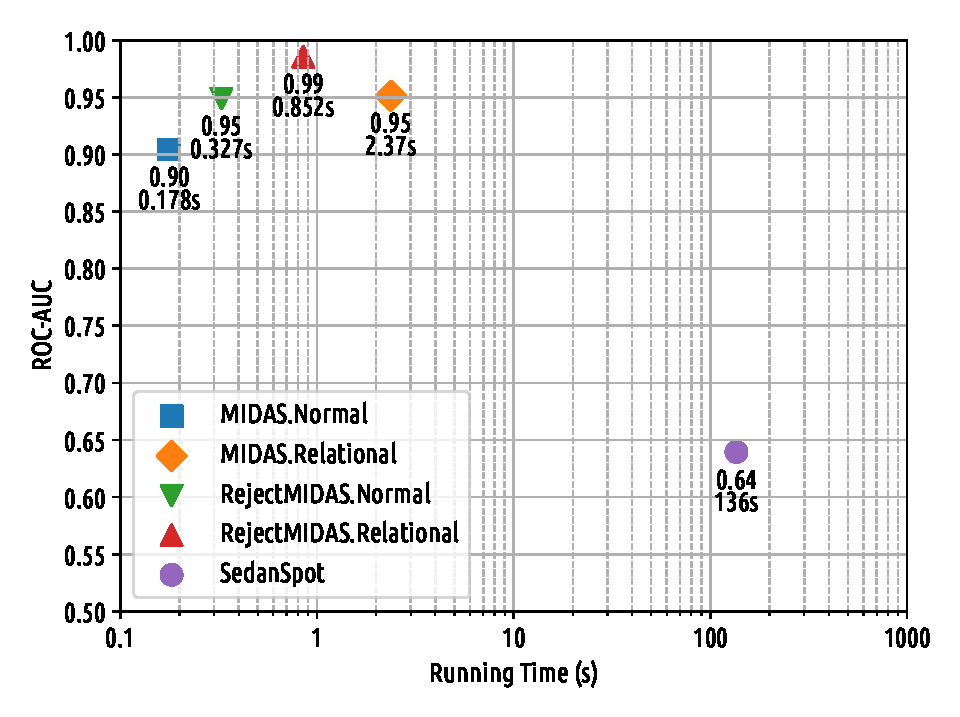
\includegraphics[width=0.5\textwidth]{img/TimeAUC.Darpa.pdf}} \\
		\subfloat[DDoS Dataset]{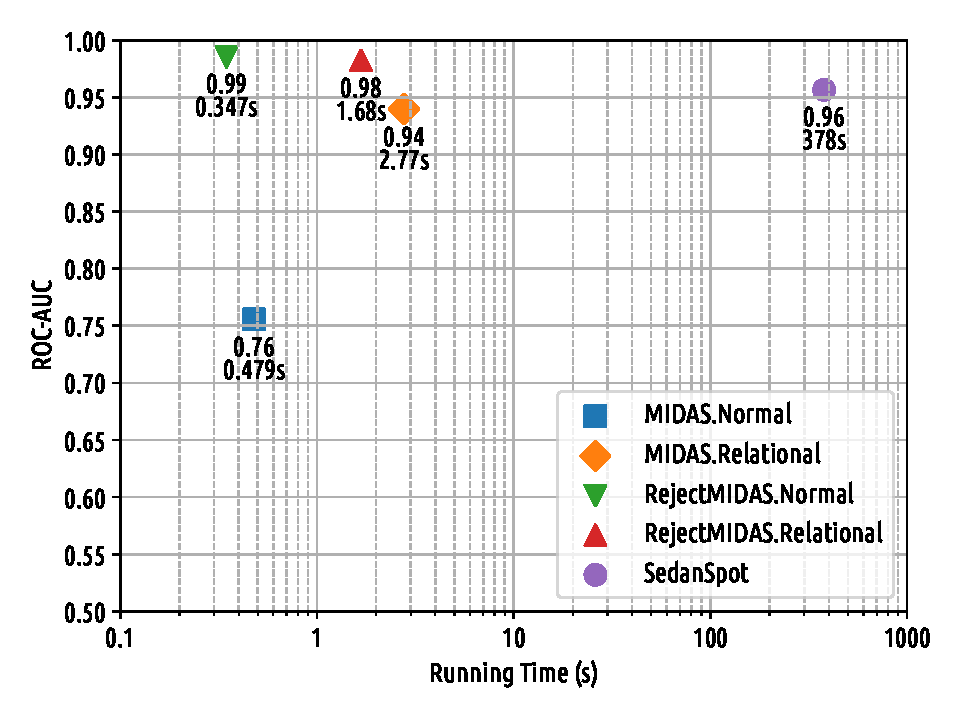
\includegraphics[width=0.5\textwidth]{img/TimeAUC.DDoS.pdf}}
		\caption{ROC-AUC metric and running time}\label{fig:TimeAUC.Darpa}
	\end{figure}

	Fig.~\ref{fig:TimeAUC.Darpa} shows the ROC-AUC vs. running time (I/O not included) on the two datasets. On the DARPA dataset, both RejectMIDAS algorithms choose 1000 as the threshold; while on the DDoS dataset, the best thresholds are 100000 and 10000, respectively. In the following experiments, if unspecified, we will reuse these thresholds as the parameter.

	On the DARPA dataset, the normal version of RejectMIDAS achieves higher AUC (0.95) than the baselines (0.9) with a small cost of running time ($+0.149s$); the relational version achieves a higher AUC (0.99 vs. 0.95) while at the same time runs even faster than the original MIDAS ($-1.52s$). Compared with SedanSpot, two RejectMIDAS algorithms increase the AUC by 48\% and 55\% and are $416\times$ and $159\times$ faster.

	On the DDoS dataset, the situation is slightly different. The normal MIDAS achieves a poor result (0.76 vs. 0.99) but runs even slower ($+0.132s$) than the RejectMIDAS. For the relational version, it resembles DARPA's situation, RejectMIDAS is faster ($-1.09s$) and more accurate (0.98 vs. 0.94) than the baseline. For the comparison between RejectMIDAS and SedanSpot, though the latter also obtains a high AUC, its slow running speed makes it infeasible to be used in a real-time situation.

	\subsection{Discussion}

	\begin{figure}[!htb]
		\centering
		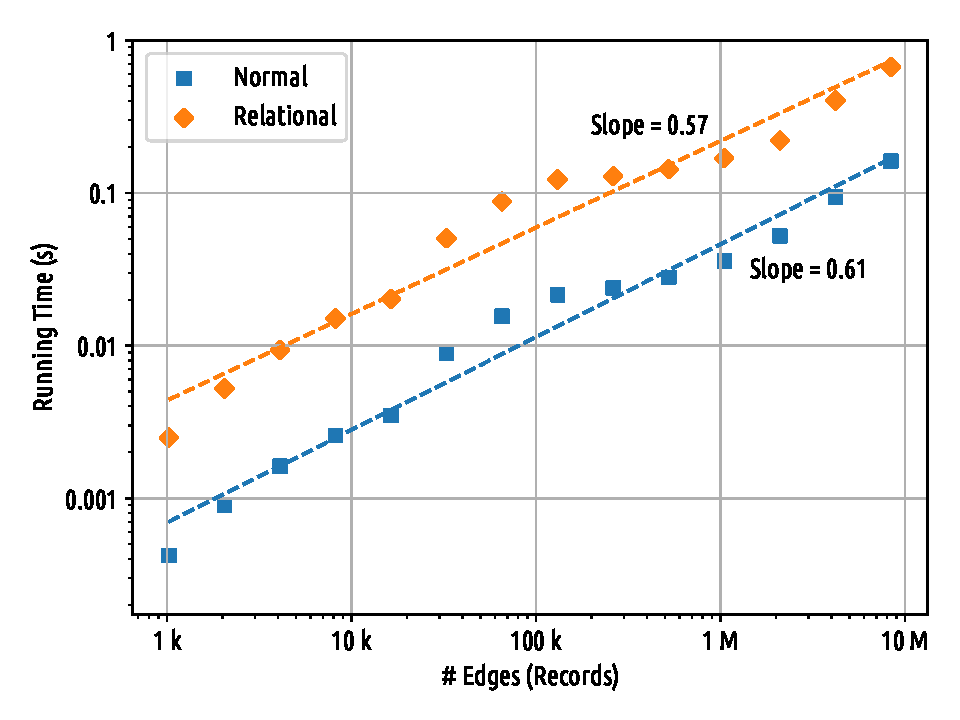
\includegraphics[width=0.5\textwidth]{img/Scalability.Edge.pdf}
		\caption{Edge Scalability}\label{fig:Scalability.Edge}
	\end{figure}

	Fig.~\ref{fig:Scalability.Edge} shows the scalability of the two RejectMIDAS algorithms. We fix the CMSs' layout to 2 rows by 1024 buckets (columns), then count the time needed to run on the first $2^{10}, \ldots, 2^{23}$ edges of the DDoS dataset. This confirms that given a constant CMS layout, two RejectMIDAS algorithms scale linearly concerning the number of edges.

	\begin{figure}[!htb]
		\centering
		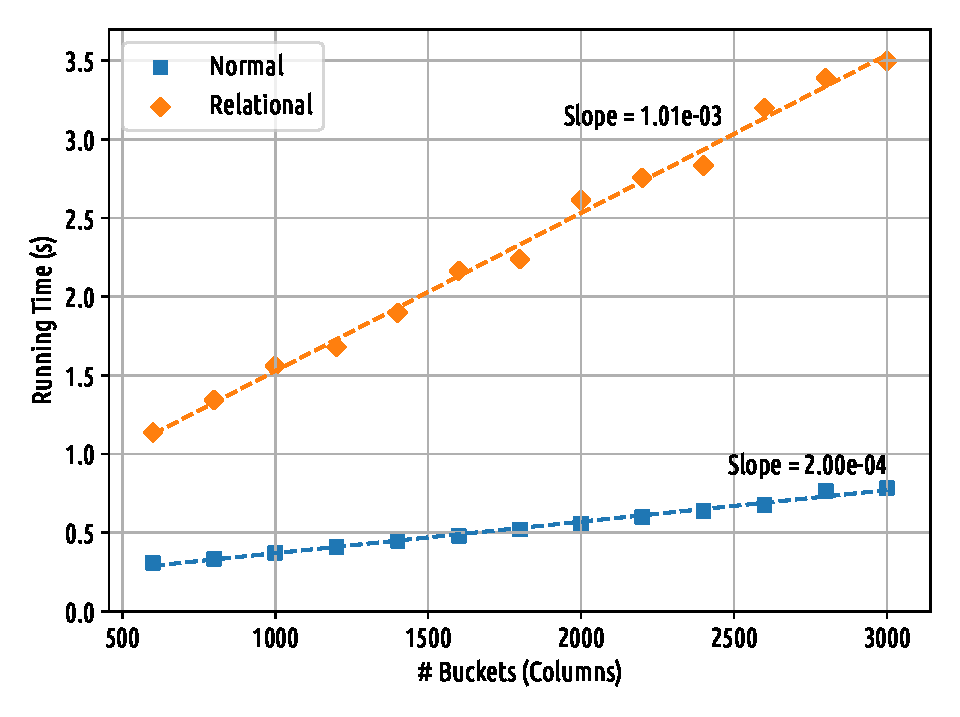
\includegraphics[width=0.5\textwidth]{img/Scalability.Bucket.pdf}
		\caption{Influence from the number of buckets}\label{fig:Scalability.Bucket}
	\end{figure}

	Fig.~\ref{fig:Scalability.Bucket} shows the bucket scalability of the RejectMIDAS algorithms. Each CMS is still 2 rows, but the number of buckets (columns) varies from 600 to 3000, with step length 200. We run the two algorithms on the DDoS dataset. This demonstrates that given a constant input, the algorithms scale linearly with respect to the length of CMSs.

	\begin{figure}[!htb]
		\centering
		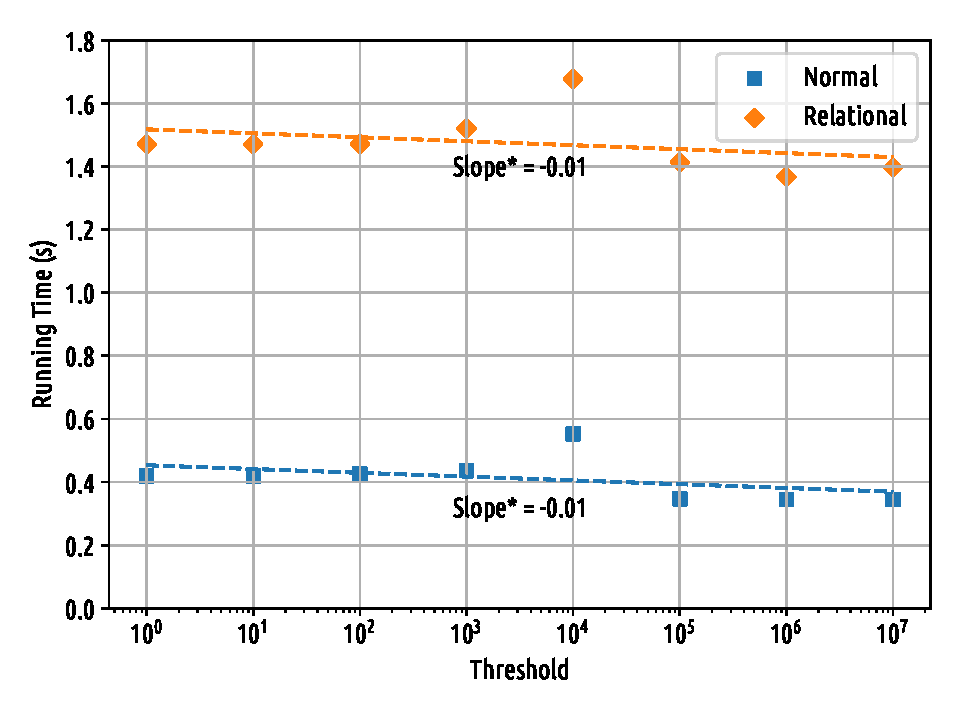
\includegraphics[width=0.5\textwidth]{img/Scalability.Threshold.pdf}
		\caption{Influence from the threshold}\label{fig:Scalability.Threshold}
	\end{figure}

	We also tested if different thresholds affect the running time. The result is shown in Fig.~\ref{fig:Scalability.Threshold}, where the slope is the ratio of running time change to log10 of threshold change. We can see that the threshold can hardly affect the running time, with an exception when the threshold is 10000.

	\begin{figure}[!htb]
		\centering
		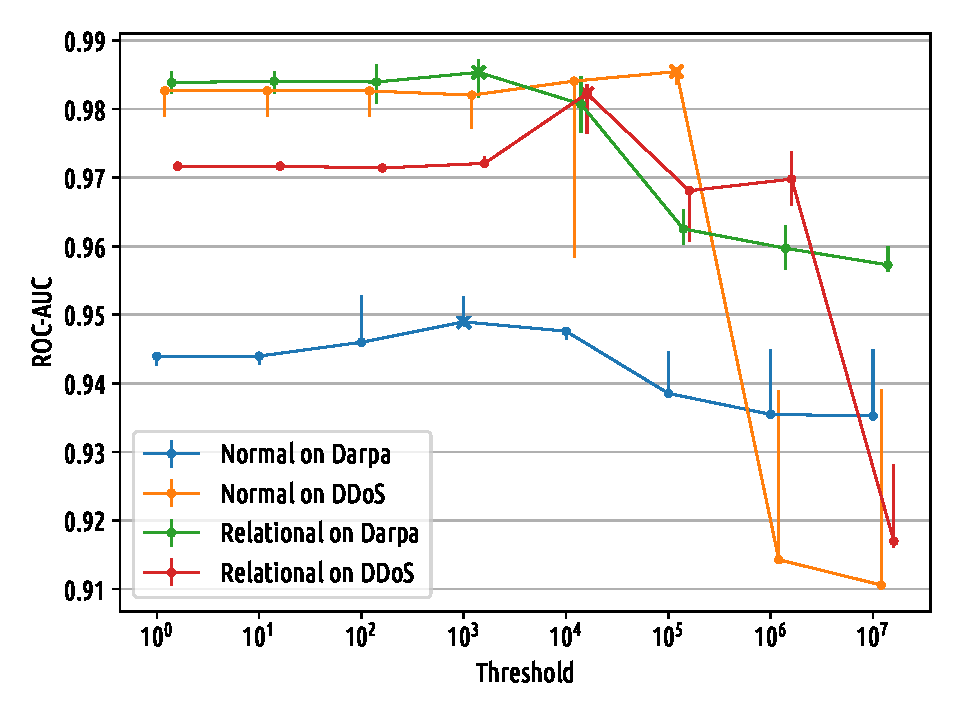
\includegraphics[width=0.5\textwidth]{img/Distribution.pdf}
		\caption{Result Distribution}\label{fig:Distribution}
	\end{figure}

	To reveal the effect of different thresholds, we plot the result distribution of the experiment performed in the last subsection. As shown in Fig.~\ref{fig:Distribution}, the points are the median AUC values, and the vertical lines indicate the range of all the 21 test results. To enhance the readability, we add a small offset to the horizontal position of each point.

	From Fig.~\ref{fig:Distribution}, we can spot a trend followed by all the experiments. We split the results into two halves from the summit points, which are denoted as cross markers. On the left, the performance increase with the threshold; on the right, the opposite trend is presented.

	One possible explanation for the left half is that when the threshold is low, edges' anomaly scores will surpass this limit more often; therefore, the CMSs counting the total occurrences of edges, sources and destinations will use the previous mean value more often. When small fluctuations come to the system, they are more likely to be mistakenly regarded as anomalous.

	For the other half, when the threshold is too large, the system becomes too generous to the anomalous situations. An extreme case is when the threshold is positive infinity, where no rejection is performed, then the algorithm will partially degenerate to the original MIDAS algorithm.


	\section{Conclusion}

	In this work, we proposed two RejectMIDAS algorithms: a normal version and a relational version. In the future, we will explore other possible ways to further enhance the performance, i.e., accuracy and speed, of the RejectMIDAS algorithm.

	\bibliography{Reference}

\end{document}